\documentclass[../main.tex]{subfiles}
\begin{document}

\chapter{Is security an illusion?}
\section{Introduction}
\begin{itemize}
\item It looks like recent attacks are very complicated, but they are mostly very easy thanks to databases sitting on the web with no authentication mechanisms. Everyone has access, but they are not deliberately made insecure. 
\item Also well secured databases are at risk.
\item Many courses focussing on developing software omit the security part. This is a big part of the problem.
\end{itemize}

\section{The web security landscape}
\begin{itemize}
\item Not only big applications with sensitive information/money transactions are targeted.
\item Every simple web application can be a target. For example use server hardware to take advantage of computer resources (mining software, fileservers, botnets,...).
\item If the application contains personal data, the risks are even higher (data breach, leverage for financial gain, selling personal data, ransomware,...
\item Challenging task to build secure software.
\item More often than not, security is seen as an obstruction. An annoyance getting in the way of functionality and productivity. As a consequence of this attitude, security is often ignored until the very last moment.
\item Often penetration test in the end of the development cycle.
\item Drawbacks!
\begin{enumerate}
\item Fundamental problem? Redesign whole application?
\item All relevant threats covered?
\item Whole application covered?
\item What if new release?
\end{enumerate}
\item Security is a process, not a task! The only way to build secure applications is by making security inherent to the application.
\item Various security activities throughout the application's life cycle are necessary:
\begin{enumerate}
\item Raise security awareness among developers.
\item Secure coding guidelines (practical ways to mitigate threats), for example: OWASP guidelines.
\item Threat modeling/risk analysis (power is in the proactive nature)
\begin{enumerate}
\item enumerate potential threats
\item Asses relevance and significance of threats
\item Define how to mitigate them into the application
\end{enumerate}
\end{enumerate}
\end{itemize}

\section{The security model of the web}
\subsection{URL/URI/URN}
\begin{itemize}
\item URL, URI and URN can be used interchangeably
\begin{figure}[h!]
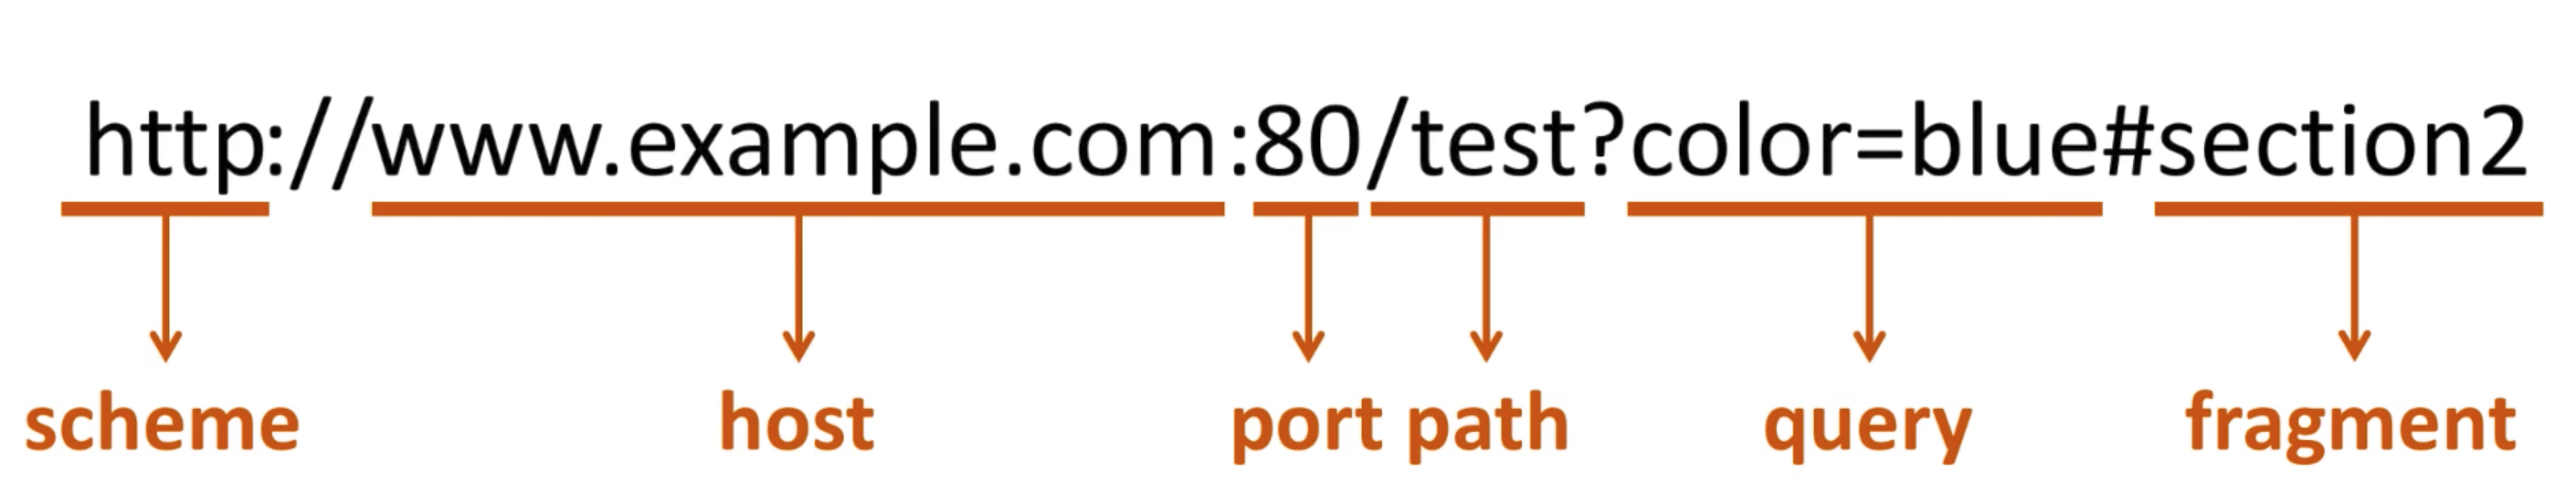
\includegraphics[width=\textwidth]{../images/url}
\caption{Naming convention of a URL}
\end{figure}
\item The \textbf{fragment} contains client side parameters. These are never sent to the server.
\item Most security decisions rely on the \textbf{origin} (scheme, host and port).
\item One of the most significant security policies: \textbf{Same-Origin Policy (SOP)}. It states that content of the same origin can freely interact with each other, while contexts from different origins are isolated.\\
Note: Two sibling applications with different paths still share the same origin, implying that they are not isolated.\\
Example: browser-provided storage mechanisms; An origin cannot access the data store of another origin.
\end{itemize}

\subsection{Cookies}
\begin{itemize}
\item With cookies, a server can send information to the browser, and the browser returns it on subsequent requests. \item Used to keep track of session information.
\item In essence, a \textbf{cookie} is nothing more than a key-value pair, separated by the equals sign. The application is free to determine both the name and value of the cookie, except for a few reserved characters.
\item The server can instruct the browser to set a cookie using the \textbf{Set-Cookie header}. The browser processes incoming Set-Cookie headers. If the headers are valid, the browsers stores the cookies in its internal storage, known as the \textbf{cookie jar}.
\item Cookies belong to a domain, and the browser consults the cookie jar for every outgoing request. If there are cookies belonging to the destination of the request, the browser automatically attaches them.
\item Requests contain cookies in the \textbf{Cookie header}.
\item Cookies are typically exchanged through HTTP headers; but the can also be accessed from JavaScript. Reading the \texttt{document.cookie} property returns the cookies from the cookie jar. The property only returns the cookies that belong to the domain of the browsing context. Cookies can also be set from JavaScript, they will will also be present on outgoing requests.
\item The server can use specific \textbf{cookie attributes} to control how the browser handles it. For example: the server can control the expiration date by setting the \textbf{Expires} attribute to a particular value.
\item A long time ago, cookies lived a short timespan, but on modern computers and phones, browser sessions can span many days or even weeks.
\item A second cookie attribute is the \textbf{Domain}, which determines the scope of the cookie. By default, cookies are only sent back to the host that sets them, but by setting the Domain attribute, the server can instruct the browser to send it to all subdomains of a particular domain.
\item For security reasons, a host can only set a cookie for its registered domain and its subdomains.
\item A third cookie attribute is the \textbf{Path} attribute, which also defines the scope of the cookie. By specifying this attribute, the server instructs the browser to only attach the cookie to requests to a resource within this path.
\item Note that the Path attribute helps prevent collisions between cookies from sibling applications.
\item Cookies belong to domains, and not on origins!
\end{itemize}

\subsection{Modern client-side focused applications}
\begin{itemize}
\item Modern web applications push a lot of responsibilities to the client.
\item Independent \textbf{frontend application}, complemented with backend services, usually provided as an API.
\item The security landscape in the early Web was vastly different from what we see today. Attackers focused their attention on server-side services.
\item As the web evolved, attackers started widening their focus as well. They discovered the potential of the browser and started using it as a conduit for their attacks.
\item All these client-side features also offer an \textbf{attractive attack surface}.
\item Modern browsers support a plethora of \textbf{security features} besides the Same-Origin Policy.
\item Example: \textbf{cookie security flags} that restrict the default behavior of cookies. The server attaches such a flag when a new cookie is set. When the browser encounters the flag, it restricts the accessibility of the cookie.
\item Cookie security flags were the precursor of a new movement in web security. They offer a security feature that is \textbf{enforced by the browser}, yet they can be \textbf{controlled by the server}.
\item The transition of the browser into an application platform sparked the need for more client-side security mechanisms $\rightarrow$ new line of security policies under control of the server, but enforced by the browser.
\item These policies are known as \textbf{server-driven browser-enforced security policies}.
\item Combining these policies with existing defences enables building a layered defence strategy.
\end{itemize}
\end{document}